\documentclass[10pt,a4papper]{article}
\usepackage{graphicx}
\usepackage{amsmath}
\usepackage{amssymb}
\usepackage{cancel}
\usepackage{multicol}
\usepackage{blindtext}
\usepackage{tikz}
\usepackage{pgfplots}
\usepackage[hidelinks]{hyperref}
\usepackage[left=2.00cm, right=3.00cm, top=2.00cm, bottom=2.00cm]{geometry}
\author{Angel Fdo. García Núñez}
\date{Enero 18, 2023}
\title{Estadisitica}

\begin{document}

\Huge
Potencial doble Delta de Dirac\\

Angel Fernando García Núñez

\Large
\newpage
\[\text{Potencial}\]
\[V(x)=-\alpha[\delta(x+a)+\delta(x-a)]\]

\begin{center}
  \begin{tikzpicture}
    \node[draw=none,above](a)at(2,0.2){$a$};
    \node[draw=none,above](ma)at(-2,0.2){$-a$}; 
    
    \draw[->] (-4,0) to (4,0) node[right]{$x$};
    \draw[->] (0,-3) to (0,1) node[above]{$V(x)$};
    \draw[line width=1pt,-stealth] (a) to (2,-3);
    \draw[line width=1pt,-stealth] (ma) to (-2,-3) ;
  \end{tikzpicture}
\end{center}\\


\[\text{Ecuación de Schrödinger Independiente del tiempo}\]

\[\hat H\psi=E\psi\quad\to\quad
-\frac{\hbar^2}{2m}\frac{d^2\psi}{dx^2}+V(x)\psi(x)=E\psi(x)\]\\

\[-\frac{\hbar^2}{2m}\frac{d^2\psi}{dx^2}-\alpha[\delta(x+a)+\delta(x-a)]\psi(x)=E\psi(x)\]\\

\[\text{Regiones sin potencial}\]

\[V(x)=0\quad:\quad |x|\not=a\]

\[-\frac{\hbar^2}{2m}\frac{d^2\psi}{dx^2}=E\psi(x)\]

\[\text{Energía menor al máximo }E<0\]

\[k\equiv\frac{\sqrt{-2mE}}{\hbar}\quad\to\quad k\in\mathbb{R}\quad:\quad E<0\]

\[\boxed{\frac{d^2\psi}{dx^2}-k^2\psi(x)=0}\]

\newpage
\[\text{Región I: }x<-a\]

\[\psi_I(x)=A'e^{-kx}+Ae^{kx}\]

\[\lim_{x\to-\infty}A'e^{-kx}\to\infty\quad\to\quad A'=0\]

\[\therefore\quad\psi_I(x)=Ae^{kx}\]\\

\[\text{Región II: }-a<x<a\]

\[\psi_{II}(x)=Ce^{-kx}+De^{kx}\]\\

\[\text{Región III: }x>a\]

\[\psi_{III}(x)=Be^{-kx}+B'e^{kx}\]

\[\lim_{x\to\infty}B'e^{kx}\to\infty\quad\to\quad B'=0\]

\[\therefore\quad\psi_{III}(x)=Be^{-kx}\]\\

\[\boxed{
  \psi(x)=
  \left\{\begin{array}{ccc}
  Ae^{kx} & : & x<-a \\
  Ce^{-kx}+De^{kx} & : & -a<x<a\\
  Be^{-kx} & : & x>a
\end{array}}\]

\newpage
\[\text{Continuidad de la función en }-a\]

\[\psi_I(-a)=\psi_{II}(-a)\]

\[Ae^{-ka}=Ce^{ka}+De^{-ka}\quad\to\quad\boxed{A=D+Ce^{2ka}}\]

\[\text{Continuidad de la función en }a\]

\[\psi_{II}(a)=\psi_{III}(a)\]

\[Ce^{-ka}+De^{ka}=Be^{-ka}\quad\to\quad\boxed{B=C+De^{2ka}}\]\\

\[\text{Derivada de }\psi(x)\]

\[\boxed{
  \frac{d\psi}{dx}=
  \left\{\begin{array}{ccc}
  kAe^{kx} & : & x<-a \\
  -kCe^{-kx}+kDe^{kx} & : & -a<x<a\\
  -kBe^{-kx} & : & x>a
\end{array}}\]

\newpage
\[\text{Integrando alrededor de }-a\]

\begin{center}
  \begin{tikzpicture}
    \node[draw=none,above](a)at(2,0.2){$a$};
    \node[draw=none,above](ma)at(-2,0.2){$-a$};
    
    \draw[->] (-4,0) to (4,0) node[right]{$x$};
    \draw[->] (0,-3) to (0,1) node[above]{$V(x)$};
    \draw[line width=1pt,-stealth] (a) to (2,-3);
    \draw[line width=1pt,-stealth] (ma) to (-2,-3) ;
    \draw[-] (-0.8,-0.1) to (-0.8,0.1) node[above]{$-a+\varepsilon$};
    \draw[-] (-3.2,-0.1) to (-3.2,0.1) node[above]{$-a-\varepsilon$};
  \end{tikzpicture}
\end{center}\\

\[-\frac{\hbar^2}{2m}\int_{-a-\varepsilon}^{-a+\varepsilon}\frac{d^2\psi}{dx^2}dx
-\alpha\int_{-a-\varepsilon}^{-a+\varepsilon}[\delta(x+a)+\delta(x-a)]\psi(x)dx=
E\int_{-a-\varepsilon}^{-a+\varepsilon}\psi(x)dx\]\\

\[-\frac{\hbar^2}{2m}\int_{-a-\varepsilon}^{-a+\varepsilon}\frac{d^2\psi}{dx^2}dx
-\alpha\int_{-a-\varepsilon}^{-a+\varepsilon}\delta(x+a)\psi(x)dx
-\alpha\cancelto{0}{\int_{-a-\varepsilon}^{-a+\varepsilon}\delta(x-a)\psi(x)dx}=
E\int_{-a-\varepsilon}^{-a+\varepsilon}\psi(x)dx\]\\

\[-\frac{\hbar^2}{2m}\int_{-a-\varepsilon}^{-a+\varepsilon}\frac{d^2\psi}{dx^2}dx
-\alpha\int_{-a-\varepsilon}^{-a+\varepsilon}\delta(x+a)\psi(x)dx=
E\int_{-a-\varepsilon}^{-a+\varepsilon}\psi(x)dx\]\\

\[-\frac{\hbar^2}{2m}\left|\frac{d\psi}{dx}\right|_{-a-\varepsilon}^{-a+\varepsilon}
-\alpha\psi(-a)=
E\int_{-a-\varepsilon}^{-a+\varepsilon}\psi(x)dx\]\\

\[-\frac{\hbar^2}{2m}\left[\frac{d\psi_{II}}{dx}(-a+\varepsilon)-\frac{d\psi_I}{dx}(-a-\varepsilon)\right]
-\alpha\psi(-a)=
E\int_{-a-\varepsilon}^{-a+\varepsilon}\psi(x)dx\]

\newpage
\[-\frac{\hbar^2}{2m}\lim_{\varepsilon\to 0}\left[\frac{d\psi_{II}}{dx}(-a+\varepsilon)-\frac{d\psi_I}{dx}(-a-\varepsilon)\right]
-\alpha\psi(-a)=0\]\\

\[-\frac{\hbar^2}{2m}\lim_{\varepsilon\to 0}\left[-kCe^{-k(-a+\varepsilon)}+kDe^{k(-a+\varepsilon)}-
  kAe^{k(-a-\varepsilon)}\right]
-\alpha Ae^{-ka}=0\]\\

\[-\frac{\hbar^2}{2m}\left(-kCe^{ka}+kDe^{-ka}-kAe^{-ka}\right)-\alpha Ae^{-ka}=0\]\\

\[-Ce^{ka}+De^{-ka}-Ae^{-ka}+\frac{2m\alpha}{k\hbar^2}Ae^{-ka}=0\]\\

\[-Ce^{ka}+\left(D-A+\frac{2m\alpha}{k\hbar^2}A\right)e^{-ka}=0\]\\

\[\left[D+\left(\frac{2m\alpha}{k\hbar^2}-1\right)A\right]e^{-ka}=Ce^{ka}\]\\

\[\boxed{D+\left(\frac{2m\alpha}{k\hbar^2}-1\right)A=Ce^{2ka}}\]

\newpage
\[\text{Integrando alrededor de }a\]

\begin{center}
  \begin{tikzpicture}
    \node[draw=none,above](a)at(2,0.2){$a$};
    \node[draw=none,above](ma)at(-2,0.2){$-a$};
    
    \draw[->] (-4,0) to (4,0) node[right]{$x$};
    \draw[->] (0,-3) to (0,1) node[above]{$V(x)$};
    \draw[line width=1pt,-stealth] (a) to (2,-3);
    \draw[line width=1pt,-stealth] (ma) to (-2,-3) ;
    \draw[-] (0.8,-0.1) to (0.8,0.1) node[above]{$a-\varepsilon$};
    \draw[-] (3.2,-0.1) to (3.2,0.1) node[above]{$a+\varepsilon$};
  \end{tikzpicture}
\end{center}\\

\[-\frac{\hbar^2}{2m}\int_{a-\varepsilon}^{a+\varepsilon}\frac{d^2\psi}{dx^2}dx
-\alpha\int_{a-\varepsilon}^{a+\varepsilon}[\delta(x+a)+\delta(x-a)]\psi(x)dx=
E\int_{a-\varepsilon}^{a+\varepsilon}\psi(x)dx\]\\

\[-\frac{\hbar^2}{2m}\int_{a-\varepsilon}^{a+\varepsilon}\frac{d^2\psi}{dx^2}dx
-\alpha\cancelto{0}{\int_{a-\varepsilon}^{a+\varepsilon}\delta(x+a)\psi(x)dx}
-\alpha\int_{a-\varepsilon}^{a+\varepsilon}\delta(x-a)\psi(x)dx=
E\int_{a-\varepsilon}^{a+\varepsilon}\psi(x)dx\]\\

\[-\frac{\hbar^2}{2m}\int_{a-\varepsilon}^{a+\varepsilon}\frac{d^2\psi}{dx^2}dx
-\alpha\int_{a-\varepsilon}^{a+\varepsilon}\delta(x-a)\psi(x)dx=
E\int_{a-\varepsilon}^{a+\varepsilon}\psi(x)dx\]\\

\[-\frac{\hbar^2}{2m}\left|\frac{d\psi}{dx}\right|_{a-\varepsilon}^{a+\varepsilon}
-\alpha\psi(a)=
E\int_{a-\varepsilon}^{a+\varepsilon}\psi(x)dx\]\\

\[-\frac{\hbar^2}{2m}\left[\frac{d\psi_{III}}{dx}(a+\varepsilon)-\frac{d\psi_{II}}{dx}(a-\varepsilon)\right]
-\alpha\psi(a)=
E\int_{a-\varepsilon}^{a+\varepsilon}\psi(x)dx\]

\newpage
\[-\frac{\hbar^2}{2m}\lim_{\varepsilon\to 0}\left[\frac{d\psi_{III}}{dx}(a+\varepsilon)-\frac{d\psi_{II}}{dx}(a-\varepsilon)\right]
-\alpha\psi(a)=0\]\\


\[-\frac{\hbar^2}{2m}\lim_{\varepsilon\to 0}\left[-kBe^{-k(a+\varepsilon)}-\left(-kCe^{-k(a-\varepsilon)}+kDe^{k(a-\varepsilon)}\right)\right]
-\alpha Be^{-ka}=0\]\\

\[-\frac{\hbar^2}{2m}\left(-kBe^{-ka}+kCe^{-ka}-kDe^{ka}\right)-\alpha Be^{-ka}=0\]\\

\[-Be^{-ka}+Ce^{-ka}-De^{ka}+\frac{2m\alpha}{k\hbar^2}Be^{-ka}=0\]\\

\[-De^{ka}+\left(C-B+\frac{2m\alpha}{k\hbar^2}B\right)e^{-ka}=0\]\\

\[\left[C+\left(\frac{2m\alpha}{k\hbar^2}-1\right)B\right]e^{-ka}=De^{ka}\]\\

\[\boxed{C+\left(\frac{2m\alpha}{k\hbar^2}-1\right)B=De^{2ka}}\]

\newpage
\[\text{Sistema de 4 ecuaciónes}\]

\[A=D+Ce^{2ka}\]

\[B=C+De^{2ka}\]

\[D+\left(\frac{2m\alpha}{k\hbar^2}-1\right)A=Ce^{2ka}\]

\[C+\left(\frac{2m\alpha}{k\hbar^2}-1\right)B=De^{2ka}\]\\

\[D+\left(\frac{2m\alpha}{k\hbar^2}-1\right)\left(D+Ce^{2ka}\right)=Ce^{2ka}\quad\to\quad
\frac{2m\alpha}{k\hbar^2}\left(D+Ce^{2ka}\right)=2Ce^{2ka}\]

\[\boxed{\frac{m\alpha}{k\hbar^2}\left(D+Ce^{2ka}\right)=Ce^{2ka}}\]\\

\[C+\left(\frac{2m\alpha}{k\hbar^2}-1\right)\left(C+De^{2ka}\right)=De^{2ka}\quad\to\quad
\frac{2m\alpha}{k\hbar^2}\left(C+De^{2ka}\right)=2De^{2ka}\]

\[\boxed{\frac{m\alpha}{k\hbar^2}\left(C+De^{2ka}\right)=De^{2ka}}\]\\

\[\frac{m\alpha}{k\hbar^2}\left(D+Ce^{2ka}\right)=Ce^{2ka}\quad\to\quad
\frac{m\alpha}{k\hbar^2}D=\left(1-\frac{m\alpha}{k\hbar^2}\right)Ce^{2ka}\]\\

\[D=\frac{k\hbar^2}{m\alpha}\left(1-\frac{m\alpha}{k\hbar^2}\right)Ce^{2ka}=
\left(\frac{k\hbar^2}{m\alpha}-1\right)Ce^{2ka}\]

\newpage
\[\frac{m\alpha}{k\hbar^2}\left(C+De^{2ka}\right)=De^{2ka}\quad\to\quad
\left(\frac{m\alpha}{k\hbar^2}-1\right)De^{2ka}+\frac{m\alpha}{k\hbar^2}C=0\]\\

\[\left(\frac{m\alpha}{k\hbar^2}-1\right)\left(\frac{k\hbar^2}{m\alpha}-1\right)Ce^{4ka}+\frac{m\alpha}{k\hbar^2}C=0\quad\to\quad
-\left(\frac{m\alpha}{k\hbar^2}+\frac{k\hbar^2}{m\alpha}-2\right)e^{4ka}+\frac{m\alpha}{k\hbar^2}=0\]\\

\[\frac{m\alpha}{k\hbar^2}\left(\frac{m\alpha}{k\hbar^2}+\frac{k\hbar^2}{m\alpha}-2\right)e^{4ka}-\left(\frac{m\alpha}{k\hbar^2}\right)^2=0\quad\to\quad
\left[\left(\frac{m\alpha}{k\hbar^2}\right)^2+1-\frac{2m\alpha}{k\hbar^2}\right]e^{4ka}-\left(\frac{m\alpha}{k\hbar^2}\right)^2=0\]\\

\[\left(\frac{m\alpha}{k\hbar^2}-1\right)^2e^{4ka}-\left(\frac{m\alpha}{k\hbar^2}\right)^2=0\quad\to\quad
\left(\frac{m\alpha}{k\hbar^2}-1\right)^2e^{4ka}=\left(\frac{m\alpha}{k\hbar^2}\right)^2\]\\

\[\left(\frac{m\alpha}{k\hbar^2}-1\right)e^{2ka}=\pm\frac{m\alpha}{k\hbar^2}\quad\to\quad
\left(\frac{m\alpha}{\hbar^2}-k\right)e^{2ka}=\pm\frac{m\alpha}{\hbar^2}\quad\to\quad
k=\frac{m\alpha}{\hbar^2}\mp\frac{m\alpha}{\hbar^2}e^{-2ka}\]\\

\[\boxed{k_\pm=\frac{m\alpha}{\hbar^2}\left(1\pm e^{-2k_\pm a}\right)}\]

\newpage
\[\text{Normalización}\]

\[\psi_\pm(x)=
\left\{\begin{array}{ccc}
Ae^{k_\pm x} & : & x<-a \\
Ce^{-k_\pm x}+De^{k_\pm x} & : & -a<x<a\\
Be^{-k_\pm x} & : & x>a
\end{array}\]\\

\[\int_{-\infty}^\infty|\psi_\pm(x)|^2dx=1\]

\[\int_{-\infty}^{-a}|\psi_{\pm I}|^2dx+\int_{-a}^a|\psi_{\pm II}|^2dx+\int_a^\infty|\psi_{\pm III}|^2dx=1\]\\

\[A^2\int_{-\infty}^{-a}e^{2k_\pm x}dx+\int_{-a}^a\left(Ce^{-k_\pm x}+De^{k_\pm x}\right)^2dx+B^2\int_a^\infty e^{-2k_\pm x}dx=1\]\\

\[A^2\int_{-\infty}^{-a}e^{2k_\pm x}dx
+C^2\int_{-a}^ae^{-2k_\pm x}dx
+D^2\int_{-a}^ae^{2k_\pm x}dx
+2CD\int_{-a}^adx
+B^2\int_a^\infty e^{-2k_\pm x}dx=1\]\\

\[\frac{A^2}{2k_\pm}\left|e^{2k_\pm x}\right|_{-\infty}^{-a}
-\frac{C^2}{2k_\pm}\left|e^{-2k_\pm x}\right|_{-a}^a
+\frac{D^2}{2k_\pm}\left|e^{2k_\pm x}\right|_{-a}^a
+2CD|x|_{-a}^a
-\frac{B^2}{2k_\pm}\left|e^{-2k_\pm x}\right|_a^\infty=1\]

\[A^2\left|e^{2k_\pm x}\right|_{-\infty}^{-a}
-C^2\left|e^{-2k_\pm x}\right|_{-a}^a
+D^2\left|e^{2k_\pm x}\right|_{-a}^a
+4k_\pm CD|x|_{-a}^a
-B^2\left|e^{-2k_\pm x}\right|_a^\infty=2k_\pm\]

\[A^2e^{-2k_\pm a}
-C^2\left(e^{-2k_\pm a}-e^{2k_\pm a}\right)
+D^2\left(e^{2k_\pm a}-e^{-2k_\pm a}\right)
+8k_\pm aCD
+B^2e^{-2k_\pm a}=2k_\pm\]

\[\left(A^2+B^2\right)e^{-2k_\pm a}
+\left(C^2+D^2\right)\left(e^{2k_\pm a}-e^{-2k_\pm a}\right)
+8k_\pm aCD=2k_\pm\]

\newpage
\[\text{Solucón para }k_+\]

\[k_+=\frac{m\alpha}{\hbar^2}\left(1+e^{-2k_+ a}\right)\]

\[A=B\quad,\quad C=D\]

\[C=\frac{A}{1+e^{2k_+ a}}\]

\[2A^2e^{-2k_+ a}+2C^2\left(e^{2k_+ a}-e^{-2k_+ a}\right)+8k_+ aC^2=2k_+\]

\[A^2e^{-2k_+ a}+C^2\left(e^{2k_+ a}-e^{-2k_+ a}\right)+4k_+ aC^2=k_+\]

\[A^2e^{-2k_+ a}+\frac{A^2}{(1+e^{2k_+ a})^2}\left(e^{2k_+ a}-e^{-2k_+ a}\right)+\frac{4k_+ aA^2}{(1+e^{2k_+ a})^2}=k_+\]

\[A^2e^{-2k_+ a}(1+e^{2k_+ a})^2+A^2\left(e^{2k_+ a}-e^{-2k_+ a}\right)+4k_+ aA^2=k_+(1+e^{2k_+ a})^2\]

\[A^2(e^{-k_+ a}+e^{k_+ a})^2+A^2\left(e^{2k_+ a}-e^{-2k_+ a}\right)+4k_+ aA^2=k_+(1+e^{2k_+ a})^2\]

\[A^2(e^{-2k_+ a}+e^{2k_+ a}+2)+A^2\left(e^{2k_+ a}-e^{-2k_+ a}\right)+4k_+ aA^2=k_+(1+e^{2k_+ a})^2\]

\[A^2\left[(e^{-2k_+ a}+e^{2k_+ a}+2)+\left(e^{2k_+ a}-e^{-2k_+ a}\right)+4k_+ a\right]=k_+(1+e^{2k_+ a})^2\]

\[A^2\left(2e^{2k_+ a}+2+4k_+ a\right)=k_+(1+e^{2k_+ a})^2\quad\to\quad
A^2=\frac{k_+(1+e^{2k_+ a})^2}{2\left(e^{2k_+ a}+2k_+ a+1\right)}\]

\[A\in\mathbb{R}\quad,\quad A>0\]

\[\boxed{A_+=\sqrt{\frac{k_+(1+e^{2k_+ a})^2}{2\left(e^{2k_+ a}+2k_+ a+1\right)}}}\]

\newpage
\[\text{Solucón para }k_-\]

\[k_-=\frac{m\alpha}{\hbar^2}\left(1+e^{-2k_- a}\right)\]

\[A=-B\quad,\quad C=-D\]

\[C=-\frac{A}{1-e^{2k_- a}}\]

\[2A^2e^{-2k_- a}+2C^2\left(e^{2k_- a}-e^{-2k_- a}\right)-8k_- aC^2=2k_-\]

\[A^2e^{-2k_- a}+C^2\left(e^{2k_- a}-e^{-2k_- a}\right)-4k_- aC^2=k_-\]

\[A^2e^{-2k_- a}+\frac{A^2}{(1-e^{2k_- a})^2}\left(e^{2k_- a}-e^{-2k_- a}\right)-\frac{4k_- aA^2}{(1-e^{2k_- a})^2}=k_-\]

\[A^2e^{-2k_- a}(1-e^{2k_- a})^2+A^2\left(e^{2k_- a}-e^{-2k_- a}\right)-4k_- aA^2=k_-(1-e^{2k_- a})^2\]

\[A^2(e^{-k_- a}-e^{k_- a})^2+A^2\left(e^{2k_- a}-e^{-2k_- a}\right)-4k_- aA^2=k_-(1-e^{2k_- a})^2\]

\[A^2(e^{-2k_- a}+e^{2k_- a}-2)+A^2\left(e^{2k_- a}-e^{-2k_- a}\right)-4k_- aA^2=k_-(1-e^{2k_- a})^2\]

\[A^2\left[(e^{-2k_- a}+e^{2k_- a}-2)+\left(e^{2k_- a}-e^{-2k_- a}\right)-4k_- a\right]=k_-(1-e^{2k_- a})^2\]

\[A^2\left(2e^{2k_- a}-2-4k_- a\right)=k_-(1-e^{2k_- a})^2\quad\to\quad
A^2=\frac{k_-(1-e^{2k_- a})^2}{2\left(e^{2k_- a}-2k_- a-1\right)}\]

\[A\in\mathbb{R}\quad,\quad A>0\]

\[\boxed{A_-=\sqrt{\frac{k_-(1-e^{2k_- a})^2}{2\left(e^{2k_- a}-2k_- a-1\right)}}}\]

\newpage
\[\text{Función de onda}\]

\[\psi_\pm(x)=
\left\{\begin{array}{ccc}
Ae^{k_\pm x} & : & x<-a \\
\frac{\pm A}{1\pm e^{2k_\pm a}}\left(e^{-k_\pm x}\pm e^{k_\pm x}\right) & : & -a<x<a\\
\pm Ae^{-k_\pm x} & : & x>a
\end{array}\quad,\quad
E_\pm=-\frac{k_\pm^2\hbar^2}{2m}\]

\[k_\pm=\frac{m\alpha}{\hbar^2}\left(1\pm e^{-2k_\pm a}\right)\quad,\quad
A_\pm=\sqrt{\frac{k_\pm(1\pm e^{2k_\pm a})^2}{2\left(e^{2k_\pm a}\pm2k_\pm a\pm 1\right)}}\]\\

\newpage
\[\text{Solución numérica}\]

\[\beta=\frac{m}{\hbar^2}\]

\[k_\pm=\alpha\beta\left(1\pm e^{-2k_\pm a}\right)\quad\to\quad
k_\pm-\alpha\beta\left(1\pm e^{-2k_\pm a}\right)=0\]

\[E_\pm=-\frac{k_\pm^2}{2\beta}\]\\

\[\text{Método de Newton Raphson}\]

\[f(k_\pm)=k_\pm-\alpha\beta\left(1\pm e^{-2k_\pm a}\right)\quad\to\quad
f'(k_\pm)=1\pm 2a\alpha\beta e^{-2k_\pm a}\]

\[k_{\pm(n+1)}=k_{\pm(n)}-\frac{f(k_{\pm(n)})}{f'(k_{\pm(n)})}\]

\newpage
\[\text{Solución numérica}\]

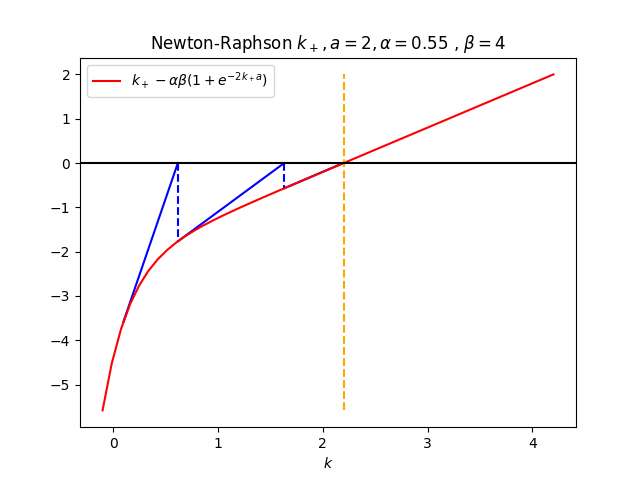
\includegraphics[height=7cm]{nrp.png}
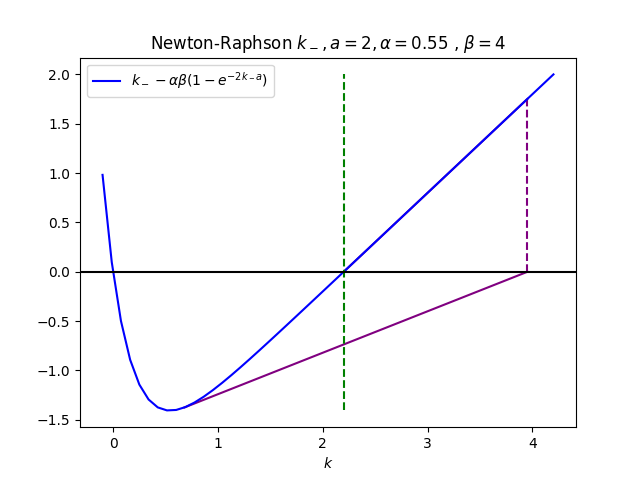
\includegraphics[height=7cm]{nrm.png}

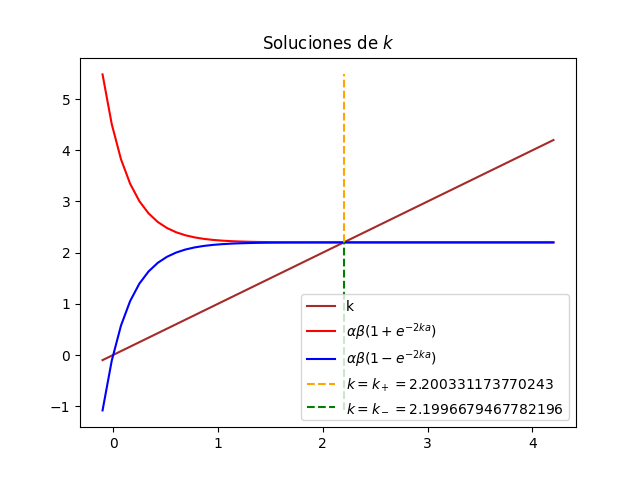
\includegraphics[height=7cm]{sol.png}
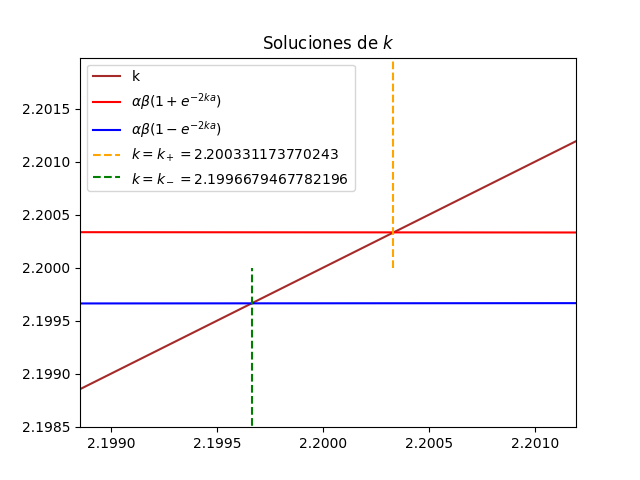
\includegraphics[height=7cm]{solz.png}

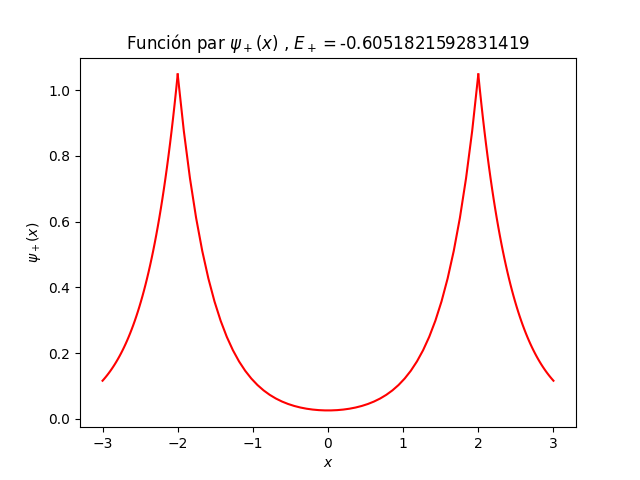
\includegraphics[height=7cm]{psip.png}
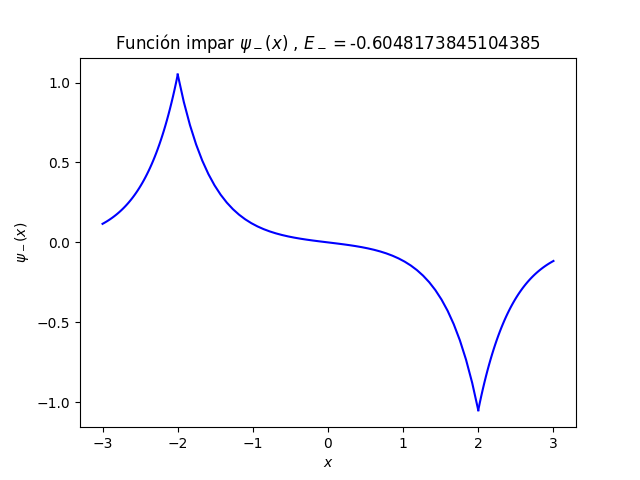
\includegraphics[height=7cm]{psim.png}

\newpage

\newpage

\newpage

\newpage

\newpage

\newpage

\newpage

\newpage

\newpage

\newpage

\newpage

\newpage

\newpage

\newpage

\newpage

\newpage

\newpage

\newpage


\end{document}
